\documentclass[12pt, a4paper, openany]{report}

% Encoding và Ngôn ngữ
\usepackage[utf8]{inputenc}
\usepackage[T5,T1]{fontenc}
\usepackage[vietnamese]{babel}

% Toán học
\usepackage{amsmath}
\usepackage{amsfonts}
\usepackage{amssymb}

% Đồ họa và Hình ảnh
\usepackage{graphicx}
\usepackage{float}
\usepackage{pdflscape}

% Bảng biểu
\usepackage{booktabs}
\usepackage{longtable}
\usepackage{array}

% Định dạng văn bản và Layout
\usepackage{geometry}
\usepackage{setspace}
\usepackage{multicol}
% \usepackage{times} % Font Times New Roman - ĐÃ VÔ HIỆU HÓA
\usepackage{sectsty}
\usepackage{enumitem}
\usepackage{caption}
\usepackage{microtype}

% Code highlighting
\usepackage{minted}

% Siêu liên kết và URL
\usepackage{hyperref}
\usepackage{xurl}

% Bibliography
\usepackage{natbib}

% Khác
\usepackage{background}
\usepackage{xcolor}
\usepackage{indentfirst}
\setlength{\parskip}{6pt plus 2pt minus 2pt}

% --- Các thiết lập cụ thể ---

\onehalfspacing

\chapterfont{\fontsize{20}{24}\selectfont\bfseries}
\sectionfont{\fontsize{16}{20}\selectfont\bfseries}
\subsectionfont{\fontsize{14}{18}\selectfont\bfseries}
\subsubsectionfont{\fontsize{12}{15}\selectfont\bfseries}

\captionsetup{labelfont=bf, skip=10pt}

\definecolor{codebg}{rgb}{0.95,0.95,0.95}
\setminted{
    bgcolor=codebg,
    fontsize=\footnotesize,
    linenos,
    frame=lines,
    framesep=2mm,
    breaklines,
    autogobble,
    python3=true, 
    breaksymbolleft={}
}

\hypersetup{
    colorlinks=true,
    linkcolor=black,
    citecolor=black,
    urlcolor=black,
    filecolor=magenta,
    pdftitle={Phân loại ảnh trên bộ dữ liệu CIFAR-10 sử dụng Mạng Nơ-ron Tích Chập (CNN)},
    pdfauthor={Người dùng},
    bookmarksnumbered=true,
    unicode=true
}

\urlstyle{same}

\backgroundsetup{
    scale=1,
    color=black,
    opacity=1,
    angle=0,
    position=current page.center,
    contents={
\includegraphics[width=\paperwidth,height=\paperheight]{background.png}}
}

\geometry{a4paper, margin=1in}

% \setlist[itemize]{itemsep=2pt}

\begin{document}

% ----- Trang bìa -----
\begin{titlepage}
\BgThispage
    \centering
    \textbf{\large HỌC VIỆN CÔNG NGHỆ BƯU CHÍNH VIỄN THÔNG}\\[0.25cm]
    \textbf{\Large KHOA CÔNG NGHỆ THÔNG TIN I}\\[0.5cm]
    \centerline{--------------------o0o--------------------}\\[1cm]
    
\includegraphics[width=8cm]{logo.png}\\[1cm]
    {\Large \textbf{BÁO CÁO BÀI TẬP LỚN 2}}\\[0.5cm]
    {\Huge \textbf{NGÔN NGỮ LẬP TRÌNH PYTHON}}\\[2cm]
\begin{center}
\begin{tabular}{@{}l@{\hspace{1.5cm}}l@{}}
\textbf{Giảng viên hướng dẫn:} & \textbf{Kim Ngọc Bách} \\
\textbf{Sinh viên:}            & \textbf{Vũ Thị Thu Duyên} \\
\textbf{Mã sinh viên:}         & \textbf{B23DCCE027} \\
\textbf{Lớp:}                  & \textbf{D23CQCEO6-B} \\
\textbf{Niên khóa:}            & \textbf{2023 - 2028} \\
\textbf{Hệ đào tạo:}           & \textbf{Đại học chính quy} \\
\end{tabular}
\end{center}
\vfill
    {\large Hà Nội, 2025}
\end{titlepage}
\backgroundsetup{contents={}}

% ----- Trang nhận xét -----
\newgeometry{top=2.5cm,bottom=2cm,left=3cm,right=2cm}

\begin{center}
    \vspace*{1cm}
    \Large\textbf{NHẬN XÉT CỦA GIẢNG VIÊN}
    \vspace{0.7cm}
\end{center}

\dotfill \vspace{0.25cm} \par
\dotfill \vspace{0.25cm} \par
\dotfill \vspace{0.25cm} \par
\dotfill \vspace{0.25cm} \par
\dotfill \vspace{0.25cm} \par
\dotfill \vspace{0.25cm} \par
\dotfill \vspace{0.25cm} \par
\dotfill \vspace{0.25cm} \par
\dotfill \vspace{0.25cm} \par
\dotfill \vspace{0.25cm} \par
\dotfill
\vspace{1.0cm}

{\textbf{\large{Điểm: }}} \hspace{1.0cm}\textbf{(Bằng chữ:} \hspace{2.5cm}\textbf{)}
\vspace{1.5cm}

\begin{flushright}
	Hà Nội, ngày \hspace{0.75cm} tháng \hspace{0.75cm} năm 20...\hspace{0.75cm}
	
	{\textbf{\large{Giảng viên  }}} \hspace{2cm} \textcolor{white}{.}
\end{flushright}
\clearpage
\restoregeometry

% ----- Mục lục, Danh sách hình ảnh -----
\tableofcontents
\cleardoublepage
\listoffigures
\cleardoublepage

% ----- Tiêu đề và Tóm tắt chính của báo cáo -----
\title{\bfseries PHÂN LOẠI ẢNH TRÊN BỘ DỮ LIỆU CIFAR-10 SỬ DỤNG MẠNG NƠ-RON TÍCH CHẬP (CNN)}
\author{}
\date{}
\maketitle

\begin{abstract}
\noindent \textbf{Nguồn dữ liệu:} CIFAR-10 dataset - \url{https://www.cs.toronto.edu/~kriz/cifar.html} \\
\textbf{Nhiệm vụ:}
\begin{itemize}
    \item Xây dựng một Mạng Nơ-ron Tích Chập (CNN) với 3 lớp tích chập.
    \item Thực hiện phân loại ảnh, bao gồm các bước huấn luyện (training), kiểm định (validation), và kiểm thử (testing).
    \item Vẽ đồ thị đường cong học tập (learning curves).
    \item Vẽ ma trận nhầm lẫn (confusion matrix).
    \item Sử dụng thư viện PyTorch.
\end{itemize}
\end{abstract}
\clearpage

% ----- Các chương nội dung -----
\chapter{Lựa chọn thư viện}
Để xây dựng và huấn luyện mạng CNN hiệu quả cho bài toán phân loại ảnh, em cần các thư viện hỗ trợ tính toán tensor linh hoạt (ưu tiên GPU nhưng có thể fallback về CPU), các lớp mạng sẵn có, thuật toán tối ưu hóa, xử lý dữ liệu ảnh và trực quan hóa kết quả.
Em lựa chọn các thư viện sau dựa trên khả năng đáp ứng yêu cầu:
\begin{itemize}
    \item \texttt{PyTorch (torch, torchvision)}: Nền tảng cốt lõi cung cấp cấu trúc tensor với khả năng tự động phát hiện và sử dụng GPU khi có sẵn, fallback về CPU khi cần thiết.
    \item \texttt{torch.nn} \& \texttt{torch.optim}: Các lớp mạng (\texttt{Conv2d}, \texttt{Linear}, \texttt{BatchNorm2d}) và thuật toán tối ưu hóa (\texttt{AdamW}, \texttt{ReduceLROnPlateau}).
    \item \texttt{torchvision.transforms}: Công cụ tiền xử lý và tăng cường dữ liệu ảnh (\texttt{Normalize}, \texttt{RandomCrop}, \texttt{RandomHorizontalFlip}).
    \item \texttt{matplotlib} \& \texttt{seaborn}: Trực quan hóa đường cong học và ma trận nhầm lẫn.
    \item \texttt{numpy} \& \texttt{sklearn}: Xử lý dữ liệu và tính toán ma trận nhầm lẫn.
    \item \texttt{time} \& \texttt{os}: Đo thời gian thực thi và quản lý file hệ thống.
    \item \texttt{multiprocessing}: Tối ưu hóa việc tải dữ liệu.
\end{itemize}

\chapter{Phương pháp thực hiện}
\section{Tiền xử lý và tăng cường dữ liệu (Data Preprocessing \& Augmentation)}
Giai đoạn đầu tiên tập trung vào việc chuẩn bị dữ liệu đầu vào từ bộ CIFAR-10. Các ảnh có kích thước 32×32 pixel với 3 kênh màu được thực hiện chuẩn hóa để đảm bảo tính ổn định trong quá trình học. Em đã áp dụng các kỹ thuật tăng cường dữ liệu bao gồm cắt ngẫu nhiên (random crop), lật ngang (horizontal flip) và xóa ngẫu nhiên một vùng ảnh (random erasing). Các phương pháp tăng cường này giúp mô hình học được các đặc trưng bất biến và giảm thiểu hiện tượng overfitting.

\section{Kiến trúc mạng CNN với 3 lớp tích chập}
Em đã xây dựng một mạng CNN gồm 3 lớp tích chập theo yêu cầu đề bài. Sau khi được tiền xử lý, dữ liệu ảnh được truyền qua chuỗi các lớp tích chập có cấu trúc phân tầng. Mỗi lớp tích chập được kết hợp với hàm kích hoạt ReLU và lớp gộp (Pooling) để tạo thành một đơn vị xử lý hoàn chỉnh. Kiến trúc này được thiết kế để trích xuất các đặc trưng theo thứ tự từ cấp độ thấp như các cạnh và góc, dần chuyển sang các đặc trưng phức tạp hơn như các bộ phận của đối tượng và hình dạng tổng thể. Để tăng cường tính ổn định và tối ưu hóa tốc độ học, em tích hợp các lớp Chuẩn hóa theo Lô (Batch Normalization) vào kiến trúc mạng.

\section{Phân loại và lớp đầu ra}
Trong giai đoạn phân loại, các đặc trưng đã được trích xuất từ 3 lớp tích chập sẽ được chuyển đổi thành vector một chiều thông qua quá trình làm phẳng (flattening). Vector đặc trưng này được xử lý qua các lớp kết nối đầy đủ (Fully Connected layers) để thực hiện phân loại cuối cùng. Để tăng cường khả năng tổng quát hóa, em tích hợp lớp Dropout nhằm kiểm soát và giảm thiểu rủi ro overfitting. Lớp đầu ra cuối cùng trả về phân phối xác suất dự đoán cho 10 lớp đối tượng trong bộ dữ liệu CIFAR-10.

\section{Huấn luyện và đánh giá}
Quá trình huấn luyện được thực hiện thông qua tối ưu hóa hàm mất mát \texttt{CrossEntropyLoss} kết hợp với kỹ thuật Label Smoothing, sử dụng thuật toán tối ưu \texttt{AdamW}. Em thực hiện huấn luyện trên tập training, theo dõi hiệu suất trên tập validation, và đánh giá cuối cùng trên tập testing.

\section{Trực quan hóa và phân tích kết quả}
Để đánh giá hiệu suất và phân tích chi tiết kết quả của mô hình, em thực hiện trực quan hóa thông qua hai phương pháp chính:
\begin{itemize}
    \item Đường cong học (Learning Curves): Vẽ đường cong loss và accuracy trên tập training và validation để theo dõi quá trình huấn luyện và phát hiện overfitting.
    \item Ma trận nhầm lẫn (Confusion Matrix): Tạo ma trận nhầm lẫn để phân tích hiệu suất phân loại trên từng lớp đối tượng và xác định các lớp thường bị nhầm lẫn.
\end{itemize}

\chapter{Quy trình triển Khai}
\section{Cấu hình}
Quá trình huấn luyện mô hình học sâu phụ thuộc vào nhiều siêu tham số và thiết lập môi trường. Em cần quản lý tập trung các cấu hình để đảm bảo tính linh hoạt, khả năng tái lập kết quả và tận dụng tối đa tài nguyên phần cứng. Em định nghĩa các cấu hình chính bao gồm:
\begin{itemize}
    \item \textbf{Cấu hình phần cứng:}
    \begin{itemize}
        \item \texttt{DEVICE}: Tự động phát hiện GPU (\texttt{cuda:0}) hoặc CPU
        \item \texttt{PIN\_MEMORY}: Tự động bật khi có GPU để tối ưu truyền dữ liệu
        \item \texttt{NUM\_WORKERS = 2}: Số tiến trình song song tải dữ liệu
    \end{itemize}
    \item \textbf{Siêu tham số huấn luyện:}
    \begin{itemize}
        \item \texttt{BATCH\_SIZE = 128}: Kích thước lô cân bằng hiệu quả và bộ nhớ
        \item \texttt{LEARNING\_RATE = 0.001}: Tốc độ học ban đầu cho AdamW
        \item \texttt{WEIGHT\_DECAY = 5e-4}: Điều chuẩn L2 được tăng để chống overfitting
        \item \texttt{NUM\_EPOCHS\_INITIAL = 300}: Số epoch tối đa cho phép
        \item \texttt{VALIDATION\_SPLIT = 0.2}: 20\% dữ liệu training dành cho validation
    \end{itemize}
    \item \textbf{Cơ chế điều chỉnh và dừng sớm:}
    \begin{itemize}
        \item \texttt{EARLY\_STOP\_PATIENCE = 5}: Dừng sớm sau 5 epoch không cải thiện validation loss
        \item \texttt{LR\_SCHEDULER\_PATIENCE = 3}: Giảm learning rate sau 3 epoch không cải thiện
    \end{itemize}
    \item \textbf{Kỹ thuật điều chuẩn:}
    \begin{itemize}
        \item \texttt{DROPOUT\_RATE = 0.5}: Tỷ lệ dropout cao để ngăn overfitting
        \item \texttt{LABEL\_SMOOTHING\_FACTOR = 0.1}: Làm mịn nhãn cải thiện tổng quát hóa
    \end{itemize}
    \item \textbf{Tính tái lập:}
    \begin{itemize}
        \item \texttt{SEED = 42}: Cố định seed đảm bảo kết quả nhất quán qua các lần chạy
    \end{itemize}
\end{itemize}

\section{Biến đổi dữ liệu (DATA TRANSFORMS)}
Dữ liệu ảnh thô gặp phải nhiều vấn đề khi đưa trực tiếp vào mô hình mạng nơ-ron. Vấn đề đầu tiên là định dạng không tương thích - mạng nơ-ron PyTorch yêu cầu đầu vào phải là các Tensor, trong khi ảnh ban đầu ở định dạng PIL hoặc NumPy array. 

Bên cạnh đó, thang giá trị pixel chưa được chuẩn hóa cũng tạo ra khó khăn trong quá trình huấn luyện. Giá trị pixel thường nằm trong khoảng [0, 255], quá lớn so với khả năng xử lý tối ưu của mạng nơ-ron. Việc chuẩn hóa về một khoảng giá trị nhỏ hơn như [0,1] hoặc [-1,1] sẽ giúp quá trình huấn luyện ổn định và nhanh hội tụ hơn. 

Vấn đề quan trọng khác là thiếu đa dạng trong tập huấn luyện. Do tập huấn luyện có kích thước hữu hạn, nếu mô hình chỉ học trên các mẫu gốc, nó dễ rơi vào tình trạng học thuộc (overfit) dữ liệu huấn luyện và hoạt động kém trên dữ liệu mới chưa từng thấy. Vì vậy, cần các kỹ thuật tăng cường để tạo ra sự đa dạng cho dữ liệu huấn luyện. 

Ngoài ra, cần phân biệt rõ ràng giữa giai đoạn huấn luyện và đánh giá. Các phép biến đổi ngẫu nhiên để tăng cường dữ liệu chỉ nên áp dụng cho tập huấn luyện, không áp dụng cho tập kiểm định và kiểm thử để đảm bảo việc đánh giá là nhất quán và khách quan.

Để giải quyết những vấn đề nêu trên, em thiết kế riêng biệt các phép biến đổi cho tập huấn luyện (\texttt{TRANSFORM\_TRAIN}) và tập kiểm định/kiểm thử (\texttt{TRANSFORM\_VAL\_TEST}) bằng \texttt{transforms.Compose} để tạo pipeline xử lý tuần tự.

\subsection{\texttt{TRANSFORM\_TRAIN} - Biến đổi cho tập huấn luyện}
Pipeline này vừa chuẩn bị định dạng dữ liệu, vừa tăng cường tính đa dạng. Em bắt đầu với \texttt{transforms.RandomCrop(32, padding=4)} - đệm 4 pixel ở mỗi cạnh rồi cắt ngẫu nhiên vùng 32x32 pixel. Điều này giúp mô hình học nhận diện đối tượng ở các vị trí khác nhau và ít nhạy cảm với sự dịch chuyển.

Sau đó, \texttt{transforms.RandomHorizontalFlip()} lật ảnh theo chiều ngang với xác suất 50\%. Kỹ thuật này hiệu quả cho CIFAR-10 vì việc lật ngang các đối tượng như ô tô, chó không làm thay đổi ý nghĩa. 

\texttt{transforms.ToTensor()} đóng vai trò then chốt, chuyển ảnh từ PIL/NumPy sang PyTorch Tensor và tự động chuẩn hóa pixel từ [0, 255] về [0.0, 1.0]. Thứ tự này quan trọng vì các bước sau yêu cầu đầu vào là Tensor. \texttt{transforms.RandomErasing(p=0.3, scale=(0.02, 0.2), ratio=(0.3, 3.3))} với xác suất 30\% sẽ xóa ngẫu nhiên một vùng hình chữ nhật trong ảnh. Kích thước vùng xóa từ 2-20\% diện tích ảnh, tỷ lệ khung hình từ 0.3-3.3. Kỹ thuật này buộc mô hình học từ các phần khác nhau của đối tượng, tăng khả năng chống che khuất. 

Cuối cùng, \texttt{transforms.Normalize((0.5, 0.5, 0.5), (0.5, 0.5, 0.5))} chuẩn hóa mỗi kênh màu về khoảng [-1.0, 1.0] bằng phép tính \texttt{(pixel - 0.5) / 0.5}. Việc chuẩn hóa này giúp quá trình huấn luyện ổn định và hội tụ nhanh hơn.

\begin{minted}{python}
TRANSFORM_TRAIN = transforms.Compose([
    transforms.RandomCrop(32, padding=4),
    transforms.RandomHorizontalFlip(),
    transforms.ToTensor(),
    transforms.RandomErasing(p=0.3, scale=(0.02, 0.2), ratio=(0.3, 3.3), value='random'),
    transforms.Normalize((0.5, 0.5, 0.5), (0.5, 0.5, 0.5))
])
\end{minted}

\subsection{\texttt{TRANSFORM\_VAL\_TEST} - Biến đổi cho tập kiểm định và kiểm thử}
Pipeline này chỉ chuẩn bị định dạng dữ liệu mà không thay đổi bản chất ảnh để đánh giá khách quan. Em chỉ sử dụng \texttt{transforms.ToTensor()} để chuyển sang Tensor và chuẩn hóa về [0.0, 1.0], sau đó \texttt{transforms.Normalize((0.5, 0.5, 0.5), (0.5, 0.5, 0.5))} để chuẩn hóa về [-1.0, 1.0]. 

Các phép tăng cường ngẫu nhiên như \texttt{RandomCrop}, \texttt{RandomHorizontalFlip}, \texttt{RandomErasing} hoàn toàn không được áp dụng. Mục đích là đánh giá hiệu năng thực sự của mô hình trên dữ liệu "sạch", đảm bảo tính nhất quán và khách quan của kết quả đánh giá.

\begin{minted}{python}
TRANSFORM_VAL_TEST = transforms.Compose([
    transforms.ToTensor(),
    transforms.Normalize((0.5, 0.5, 0.5), (0.5, 0.5, 0.5))
])
\end{minted}

\section{Định nghĩa mô hình (MODEL DEFINITION - Net)}
Mô hình em thiết kế theo nguyên tắc cân bằng giữa khả năng biểu diễn và tính thực tế. Kiến trúc đủ sâu để học các đặc trưng phức tạp nhưng không quá phức tạp để tránh overfitting và tiêu tốn quá nhiều tài nguyên. Mỗi thành phần trong kiến trúc đều có vai trò cụ thể: \texttt{BatchNorm} giúp ổn định quá trình huấn luyện, \texttt{MaxPool} tạo tính bất biến và giảm tính toán, \texttt{Dropout} chống overfitting, và cấu trúc phân cấp đảm bảo việc học đặc trưng hiệu quả từ cơ bản đến phức tạp. Thiết kế này phù hợp cho các bài toán phân loại ảnh từ cơ bản đến trung bình với khả năng mở rộng tốt.

\subsection{Cấu trúc tổng thể}
Lớp \texttt{Net} kế thừa từ \texttt{nn.Module}, bao gồm hai phần chính: ba khối tích chập để trích xuất đặc trưng và hai lớp kết nối đầy đủ để phân loại. Em thiết kế theo nguyên tắc tăng dần số kênh từ 3 đến 32, 64, rồi 128 kênh, đồng thời giảm dần kích thước không gian từ 32×32 xuống 16×16, 8×8, và cuối cùng là 4×4. Nguyên tắc này giúp mạng học được các đặc trưng từ đơn giản đến phức tạp một cách tự nhiên.

\subsection{Khối tích chập}
Khối tích chập đầu tiên \texttt{conv1} nhận ảnh RGB 3 kênh đầu vào và tạo ra 32 bản đồ đặc trưng với kernel kích thước 3×3 và \texttt{padding=1} để giữ nguyên kích thước ảnh. Lớp chuẩn hóa \texttt{bn1} được áp dụng ngay sau để chuẩn hóa phân bố dữ liệu, giúp ổn định quá trình huấn luyện và tăng tốc độ học. Lớp pooling \texttt{pool1} với kích thước 2×2 giảm kích thước ảnh đi một nửa, tạo tính bất biến với dịch chuyển và giảm khối lượng tính toán. 

Khối thứ hai có cấu trúc tương tự nhưng tăng số kênh từ 32 lên 64 để học các đặc trưng phức tạp hơn từ đầu ra của khối đầu tiên. Việc tăng số kênh này cho phép mạng có thể biểu diễn nhiều loại đặc trưng khác nhau ở mức trung gian.

Khối thứ ba tiếp tục tăng lên 128 kênh để học các đặc trưng cấp cao nhất. Sau ba lần áp dụng pooling, ảnh ban đầu 32×32 pixel được giảm xuống còn 4×4 pixel. 

Việc tăng dần số kênh theo kiến trúc này có ý nghĩa sâu sắc. Ở khối đầu, mạng chỉ cần học các đặc trưng cơ bản như cạnh và góc nên 32 kênh là đủ. Ở khối giữa, mạng cần kết hợp các cạnh để tạo thành các hình dạng phức tạp hơn nên cần 64 kênh. Ở khối cuối, mạng phải học các đặc trưng cao cấp như texture và pattern nên cần đến 128 kênh. Cách thiết kế này cho phép mạng học một cách có hệ thống và tối ưu tài nguyên tính toán.

\begin{minted}{python}
self.conv1 = nn.Conv2d(3, 32, kernel_size=3, padding=1)
self.bn1 = nn.BatchNorm2d(32)
self.pool1 = nn.MaxPool2d(kernel_size=2, stride=2)

self.conv2 = nn.Conv2d(32, 64, kernel_size=3, padding=1)
self.bn2 = nn.BatchNorm2d(64)
self.pool2 = nn.MaxPool2d(kernel_size=2, stride=2)

self.conv3 = nn.Conv2d(64, 128, kernel_size=3, padding=1)
self.bn3 = nn.BatchNorm2d(128)
self.pool3 = nn.MaxPool2d(kernel_size=2, stride=2)
\end{minted}

\subsection{Lớp phân loại}
Sau khi trích xuất đặc trưng, tensor đầu ra có kích thước \texttt{(batch\_size, 128, 4, 4)} được làm phẳng thành \texttt{(batch\_size, 2048)} để chuẩn bị cho các lớp kết nối đầy đủ. Lớp \texttt{fc1} đầu tiên chuyển đổi từ 2048 đặc trưng xuống 512 đặc trưng, kèm theo lớp chuẩn hóa \texttt{bn\_fc1} để ổn định quá trình học. 

Em áp dụng dropout chỉ ở lớp kết nối đầy đủ vì đây là nơi có số lượng tham số lớn nhất, do đó có nguy cơ overfitting cao nhất. Các lớp tích chập do có cơ chế chia sẻ trọng số nên ít bị overfitting hơn. Lớp \texttt{fc2} cuối cùng tạo ra logits cho từng lớp phân loại, với số lượng đầu ra bằng \texttt{num\_classes}.

\begin{minted}{python}
self.fc1 = nn.Linear(128 * 4 * 4, 512)
self.bn_fc1 = nn.BatchNorm1d(512)
self.dropout = nn.Dropout(dropout_rate)
self.fc2 = nn.Linear(512, num_classes)
\end{minted}

\subsection{Luồng xử lý (Forward Pass)}
Dữ liệu đi qua ba khối tích chập theo pattern cố định: \texttt{Convolution -> BatchNorm -> ReLU -> MaxPool}, trong đó em chọn hàm kích hoạt ReLU vì nó tính toán nhanh, đơn giản và giúp tránh vấn đề vanishing gradient trong quá trình huấn luyện. Sau khi đi qua ba khối trích xuất đặc trưng, dữ liệu được làm phẳng và đi qua hai lớp kết nối đầy đủ với dropout được áp dụng ở giữa để chống overfitting. Đầu ra cuối cùng là tensor logits sẽ được xử lý bởi hàm loss \texttt{CrossEntropyLoss}, hàm này đã tích hợp sẵn Softmax để tính xác suất và loss cho quá trình huấn luyện.

\begin{minted}{python}
def forward(self, x):
    x = self.pool1(F.relu(self.bn1(self.conv1(x))))
    x = self.pool2(F.relu(self.bn2(self.conv2(x))))
    x = self.pool3(F.relu(self.bn3(self.conv3(x))))
    x = x.view(-1, 128 * 4 * 4)
    x = F.relu(self.bn_fc1(self.fc1(x)))
    x = self.dropout(x)
    x = self.fc2(x)
    return x
\end{minted}

\section{Hàm hỗ trợ (HELPER FUNCTIONS)}
Trong quá trình phát triển chương trình huấn luyện học sâu, em nhận thấy có nhiều đoạn logic được lặp đi lặp lại hoặc thực hiện các tác vụ cụ thể, độc lập. Điều này dẫn đến việc code trở nên dài dòng và khó bảo trì. Cụ thể, cần xử lý ba vấn đề chính: việc tải và tiền xử lý dữ liệu thành các batch, quy trình thực hiện một epoch huấn luyện với các bước cố định, và quy trình đánh giá mô hình trên tập dữ liệu mà không cập nhật trọng số.

Để giải quyết các vấn đề này, em đóng gói các đoạn logic thành các hàm riêng biệt (helper functions). Cách tiếp cận này giúp mã nguồn trở nên module hóa, dễ đọc và dễ bảo trì hơn. Đồng thời, nó cho phép tái sử dụng code và làm cho hàm thực thi chính trở nên gọn gàng, tập trung vào việc điều phối chung thay vì chi tiết triển khai.

\subsection{Function \texttt{get\_dataloaders}: Chuẩn bị Pipeline Dữ liệu}
Mô hình học sâu đòi hỏi dữ liệu đầu vào phải được cung cấp theo một cách có cấu trúc và hiệu quả. Cần giải quyết được năm thách thức chính. Đầu tiên là tải dữ liệu từ nguồn một cách đáng tin cậy. Tiếp theo là phân chia tập dữ liệu gốc thành tập huấn luyện và validation để theo dõi quá trình học. Thứ ba là áp dụng các phép biến đổi phù hợp cho từng tập dữ liệu. Thứ tư là tạo các batch dữ liệu để xử lý hiệu quả trên GPU. Cuối cùng là xáo trộn dữ liệu huấn luyện để giảm phương sai gradient và giúp mô hình hội tụ tốt hơn.

Để đạt được hiệu quả tối ưu, em cần tải và tiền xử lý dữ liệu song song với quá trình tính toán GPU. PyTorch \texttt{DataLoader} kết hợp với \texttt{Dataset} và \texttt{Sampler} chính là giải pháp tối ưu cho các vấn đề này.

\subsubsection*{Logic triển khai và luồng xử lý}
\noindent\textbf{Bước 1: Đảm bảo dữ liệu có sẵn}

Em bắt đầu bằng việc tải dữ liệu CIFAR-10 về máy thông qua lệnh \texttt{download=True}, kết quả được gán cho biến "\_" vì chỉ cần đảm bảo dữ liệu tồn tại chứ không sử dụng trực tiếp. Ngay sau đó, em tạo \texttt{full\_train\_dataset} để làm việc thực tế với \texttt{download=False}, tránh tải lại không cần thiết.

\noindent\textbf{Bước 2: Phân chia dữ liệu ngẫu nhiên} 

Em thực hiện phân chia tập training gốc thành hai phần: training và validation. Đầu tiên, em tính số lượng mẫu validation dựa trên tỷ lệ đã định và sử dụng \texttt{np.floor} để đảm bảo kết quả là số nguyên.
Bước quan trọng nhất là tạo danh sách chỉ số từ 0 đến tổng số mẫu, sau đó áp dụng \texttt{np.random.shuffle} để xáo trộn ngẫu nhiên. Việc xáo trộn này đảm bảo các mẫu validation được phân bố đều trên toàn dataset, không bị thiên vị. Sau khi xáo trộn, em chia danh sách thành \texttt{val\_idx} (phần đầu) và \texttt{train\_idx} (phần còn lại).

\noindent\textbf{Bước 3: Áp dụng transform phù hợp} 

Do yêu cầu xử lý khác nhau, em tạo hai dataset riêng từ cùng nguồn dữ liệu gốc. Dataset cho training sử dụng \texttt{TRANSFORM\_TRAIN} bao gồm data augmentation như xoay, lật, thay đổi màu sắc để tăng tính đa dạng. Dataset cho validation chỉ áp dụng \texttt{TRANSFORM\_VAL\_TEST} với các phép chuẩn hóa cơ bản, không có augmentation ngẫu nhiên để đảm bảo kết quả đánh giá nhất quán.

\noindent\textbf{Bước 4: Tạo sampler chọn lọc mẫu} 

Em sử dụng \texttt{SubsetRandomSampler} để đảm bảo mỗi dataset chỉ lấy đúng những mẫu được phân bổ. \texttt{train\_sampler} chỉ lấy mẫu có chỉ số trong \texttt{train\_idx} và vẫn duy trì tính ngẫu nhiên ở mỗi epoch. \texttt{val\_sampler} hoạt động tương tự với \texttt{val\_idx}.

\noindent\textbf{Bước 5: Xây dựng DataLoader hoàn chỉnh} 

Cuối cùng, em tạo ba \texttt{DataLoader} cho các mục đích khác nhau. \texttt{trainloader} kết hợp dataset đã augment với \texttt{train\_sampler}, đảm bảo chỉ mẫu training được sử dụng với transform phù hợp. \texttt{valloader} làm tương tự với dataset chuẩn hóa và \texttt{val\_sampler}.

\texttt{testloader} được tạo riêng từ tập test gốc của CIFAR-10 với \texttt{train=False} và \texttt{shuffle=False} vì thứ tự không quan trọng trong đánh giá cuối. Tất cả \texttt{DataLoader} đều được tối ưu với \texttt{num\_workers} và \texttt{pin\_memory} để xử lý song song và tăng tốc truyền dữ liệu lên GPU.

Kết quả là một pipeline dữ liệu hoàn chỉnh: \texttt{trainloader} với augmentation cho huấn luyện, \texttt{valloader} với transform cơ bản cho validation, và \texttt{testloader} cho đánh giá cuối cùng.

\begin{minted}{python}
def get_dataloaders(batch_size, num_workers, pin_memory, validation_split):
    _ = torchvision.datasets.CIFAR10(root='./data', train=True, download=True)
    full_train_dataset = torchvision.datasets.CIFAR10(root='./data', train=True, download=False)

    num_train_val = len(full_train_dataset)
    indices = list(range(num_train_val))
    split = int(np.floor(validation_split * num_train_val))
    np.random.shuffle(indices)
    train_idx, val_idx = indices[split:], indices[:split]

    train_dataset = torchvision.datasets.CIFAR10(root='./data', train=True, transform=TRANSFORM_TRAIN, download=False)
    val_dataset = torchvision.datasets.CIFAR10(root='./data', train=True, transform=TRANSFORM_VAL_TEST, download=False)

    train_sampler = torch.utils.data.SubsetRandomSampler(train_idx)
    val_sampler = torch.utils.data.SubsetRandomSampler(val_idx)

    trainloader = torch.utils.data.DataLoader(train_dataset, batch_size=batch_size, sampler=train_sampler, num_workers=num_workers, pin_memory=pin_memory)
    valloader = torch.utils.data.DataLoader(val_dataset, batch_size=batch_size, sampler=val_sampler, num_workers=num_workers, pin_memory=pin_memory)

    test_dataset = torchvision.datasets.CIFAR10(root='./data', train=False, transform=TRANSFORM_VAL_TEST, download=True)
    testloader = torch.utils.data.DataLoader(test_dataset, batch_size=batch_size, shuffle=False, num_workers=num_workers, pin_memory=pin_memory)
    return trainloader, valloader, testloader
\end{minted}

\subsection{Hàm \texttt{train\_one\_epoch}: Thực hiện một epoch huấn luyện hoàn chỉnh}
Hàm này chịu trách nhiệm thực hiện một lượt huấn luyện đầy đủ trên toàn bộ dữ liệu trong \texttt{trainloader}, bao gồm việc cập nhật trọng số mô hình và theo dõi các chỉ số hiệu năng. Dưới đây là phần logic xử lý từng bước một cách có hệ thống:

\subsubsection*{Chuẩn bị mô hình và khởi tạo biến theo dõi}
Em bắt đầu bằng việc chuyển mô hình sang chế độ huấn luyện thông qua \texttt{model.train()}, điều này quan trọng vì Dropout sẽ được kích hoạt và \texttt{BatchNorm2d} sẽ cập nhật thống kê dựa trên dữ liệu hiện tại. Đồng thời, em khởi tạo các biến \texttt{running\_loss}, \texttt{correct\_train}, và \texttt{total\_train} để theo dõi hiệu năng tổng thể của epoch.

\subsubsection*{Xử lý từng lô dữ liệu theo chuỗi bước chuẩn}
Với mỗi lô từ \texttt{trainloader}, em thực hiện quy trình bốn bước chính. Đầu tiên, chuyển \texttt{inputs} và \texttt{labels} lên \texttt{device} để đảm bảo tính nhất quán. Tiếp theo, gọi \texttt{optimizer.zero\_grad()} để xóa gradient từ lô trước vì PyTorch tích lũy gradient mặc định.

Sau đó, em thực hiện forward pass qua \texttt{outputs = model(inputs)} và tính mất mát bằng \texttt{loss = criterion(outputs, labels)}. Cuối cùng, \texttt{loss.backward()} tính gradient thông qua backpropagation và \texttt{optimizer.step()} cập nhật trọng số theo hướng giảm thiểu mất mát.

\subsubsection*{Thu thập thống kê và tính toán độ chính xác}
Trong quá trình xử lý, em liên tục cập nhật các chỉ số theo dõi. Mất mát được tích lũy bằng cách nhân \texttt{loss.item()} với kích thước lô để đảm bảo tính toán chính xác khi lô có thể khác nhau về kích thước.
Để đánh giá độ chính xác, em sử dụng \texttt{torch.max(outputs.data, 1)} tìm lớp có điểm cao nhất làm dự đoán, sau đó so sánh với nhãn thực tế để đếm số dự đoán đúng và cập nhật tổng số mẫu.

\subsubsection*{Tính toán kết quả cuối epoch}
Khi hoàn thành tất cả các lô, em tính mất mát trung bình bằng cách chia tổng mất mát cho tổng số mẫu, và độ chính xác bằng tỷ lệ phần trăm dự đoán đúng. Hàm trả về \texttt{epoch\_loss} và \texttt{epoch\_acc} để cung cấp cái nhìn tổng quan về hiệu năng mô hình, đồng thời kiểm tra \texttt{total\_train > 0} để tránh lỗi chia cho 0.

\begin{minted}{python}
def train_one_epoch(model, trainloader, criterion, optimizer, device):
    model.train()
    running_loss = 0.0
    correct_train = 0
    total_train = 0
    for inputs, labels in trainloader:
        inputs, labels = inputs.to(device), labels.to(device)
        optimizer.zero_grad()
        outputs = model(inputs)
        loss = criterion(outputs, labels)
        loss.backward()
        optimizer.step()
        running_loss += loss.item() * inputs.size(0)
        _, predicted = torch.max(outputs.data, 1)
        total_train += labels.size(0)
        correct_train += (predicted == labels).sum().item()
    epoch_loss = running_loss / total_train if total_train > 0 else 0.0
    epoch_acc = 100 * correct_train / total_train if total_train > 0 else 0.0
    return epoch_loss, epoch_acc
\end{minted}

\subsection{Hàm \texttt{validate\_one\_epoch(model, valloader, criterion, device)}}
Hàm \texttt{validate\_one\_epoch} đánh giá hiệu năng mô hình trên tập validation sau mỗi epoch huấn luyện. Quá trình này không chỉ giúp theo dõi overfitting thông qua việc so sánh hiệu năng giữa tập huấn luyện và validation, mà còn cung cấp thông tin quan trọng để điều chỉnh siêu tham số như learning rate scheduling và early stopping. Đồng thời, kết quả validation là cơ sở để lưu trữ mô hình có hiệu năng tốt nhất.

\subsubsection*{Chuẩn bị mô hình cho quá trình đánh giá}
Trước khi bắt đầu đánh giá, em thực hiện \texttt{model.eval()} để chuyển mô hình sang chế độ evaluation. Điều này thay đổi hành vi của các lớp đặc biệt: Dropout ngừng vô hiệu hóa nơ-ron, BatchNorm sử dụng running statistics thay vì tính từ batch hiện tại. Sau đó, em khởi tạo các biến theo dõi \texttt{running\_loss = 0.0}, \texttt{correct\_val = 0}, \texttt{total\_val = 0} để tích lũy kết quả trong suốt quá trình đánh giá.

\subsubsection*{Thực hiện đánh giá với \texttt{torch.no\_grad()}}
Em sử dụng \texttt{torch.no\_grad()} để tạo môi trường không theo dõi gradient, giúp tiết kiệm bộ nhớ và tăng tốc độ xử lý. Trong khối này, em lặp qua từng batch từ \texttt{valloader}, chuyển dữ liệu lên \texttt{device} phù hợp, sau đó thực hiện forward pass để lấy predictions. Với mỗi batch, em tính loss bằng \texttt{criterion} và tích lũy vào \texttt{running\_loss}, đồng thời sử dụng \texttt{torch.max()} để tìm class dự đoán có xác suất cao nhất.

\subsubsection*{Tính toán và trả về kết quả}
Để đánh giá độ chính xác, em so sánh predictions với nhãn thực tế và đếm số dự đoán đúng. Cuối cùng, em tính toán hai chỉ số quan trọng: \texttt{epoch\_loss = running\_loss / total\_val} thể hiện mức độ sai lệch trung bình, và \texttt{epoch\_acc = 100 * correct\_val / total\_val} cho biết tỷ lệ phần trăm dự đoán đúng. Cả hai tính toán đều có điều kiện kiểm tra \texttt{total\_val > 0} để tránh lỗi chia cho 0. Hàm trả về tuple \texttt{(epoch\_loss, epoch\_acc)} cung cấp cái nhìn toàn diện về hiệu năng mô hình, là cơ sở để đưa ra quyết định trong quá trình huấn luyện.

\begin{minted}{python}
def validate_one_epoch(model, valloader, criterion, device):
    model.eval()
    running_loss = 0.0
    correct_val = 0
    total_val = 0
    with torch.no_grad():
        for inputs, labels in valloader:
            inputs, labels = inputs.to(device), labels.to(device)
            outputs = model(inputs)
            loss = criterion(outputs, labels)
            running_loss += loss.item() * inputs.size(0)
            _, predicted = torch.max(outputs.data, 1)
            total_val += labels.size(0)
            correct_val += (predicted == labels).sum().item()
    epoch_loss = running_loss / total_val if total_val > 0 else 0.0
    epoch_acc = 100 * correct_val / total_val if total_val > 0 else 0.0
    return epoch_loss, epoch_acc
\end{minted}

\section{Hàm vẽ biểu đồ (PLOTTING FUNCTIONS)}
Trong quá trình huấn luyện mô hình, việc chỉ nhìn vào các con số về mất mát và độ chính xác qua từng epoch thường không đủ để hiểu rõ toàn cảnh quá trình học. Các giá trị số này, dù chính xác, nhưng khó phát hiện những vấn đề tiềm ẩn trong mô hình. 

Chính vì vậy, em cần đến các công cụ trực quan hóa để có thể chẩn đoán hiệu quả hơn. Thông qua biểu đồ, em có thể nhanh chóng nhận biết các hiện tượng như overfitting - khi mô hình học quá tốt trên dữ liệu huấn luyện nhưng kém trên dữ liệu kiểm định, hoặc underfitting - khi hiệu năng trên cả hai tập đều thấp. Bên cạnh đó, việc phân tích ma trận nhầm lẫn giúp em hiểu rõ mô hình thường nhầm lẫn giữa những lớp nào, từ đó có hướng cải thiện phù hợp.

\subsection{Hàm vẽ learning curves}
Để giải quyết nhu cầu này, em phát triển hàm \texttt{plot\_learning\_curves()} với mục đích hiển thị quá trình học của mô hình qua từng epoch thông qua hai biểu đồ quan trọng.
\begin{itemize}
    \item \textbf{Biểu đồ Loss:} Theo dõi quá trình học của mô hình - loss giảm dần là dấu hiệu tốt. Sự chênh lệch giữa train và validation loss giúp phát hiện overfitting.
    \item \textbf{Biểu đồ Accuracy:} Đo lường hiệu suất thực tế - cho biết mô hình dự đoán đúng bao nhiêu phần trăm. Kết hợp với loss để có cái nhìn toàn diện về chất lượng mô hình.
\end{itemize}
\textbf{Cách thức hoạt động của hàm:} \\
Hàm nhận vào lịch sử các giá trị mất mát và độ chính xác của cả tập huấn luyện và tập kiểm định, cùng với tổng số epoch đã thực hiện. Từ đó, hàm tạo ra hai đồ thị song song để so sánh. 

Đầu tiên, em tạo khung hiển thị bằng cách xác định khoảng epoch (\texttt{epochs\_range}) từ 1 đến số epoch đã chạy và thiết lập cửa sổ đồ thị kích thước 14x6 inches. Sau đó, em chia không gian hiển thị thành hai phần để vẽ đồng thời hai loại thông tin. 

Đồ thị bên trái hiển thị sự biến đổi của mất mát theo thời gian. Em vẽ hai đường cong: một cho tập huấn luyện và một cho tập kiểm định, với các nhãn, tiêu đề và lưới rõ ràng để dễ quan sát. Tương tự, đồ thị bên phải thể hiện độ chính xác theo epoch, cũng với hai đường cong tương ứng. 

Cuối cùng, em sử dụng \texttt{plt.tight\_layout()} để tự động điều chỉnh bố cục, đảm bảo các thành phần không chồng chéo và hiển thị đẹp mắt.

\begin{minted}{python}
def plot_learning_curves(train_losses, val_losses,
                         train_accuracies, val_accuracies, num_epochs_run):
    epochs_range = range(1, num_epochs_run + 1)
    plt.figure(figsize=(14, 6))
    plt.subplot(1, 2, 1)
    plt.plot(epochs_range, train_losses, label='Train Loss')
    plt.plot(epochs_range, val_losses, label='Validation Loss')
    plt.xlabel('Epochs')
    plt.ylabel('Loss')
    plt.title('Learning Curve - Loss')
    plt.legend()
    plt.grid(True)

    plt.subplot(1, 2, 2)
    plt.plot(epochs_range, train_accuracies, label='Train Accuracy')
    plt.plot(epochs_range, val_accuracies, label='Validation Accuracy')
    plt.xlabel('Epochs')
    plt.ylabel('Accuracy (%)')
    plt.title('Learning Curve - Accuracy')
    plt.legend()
    plt.grid(True)
    
    plt.tight_layout()
    plt.show()
\end{minted}

\subsection{Hàm vẽ ma trận nhầm lẫn (confusion matrix)}
Bên cạnh việc theo dõi quá trình học tổng thể, em cần hiểu rõ hơn về chất lượng dự đoán của mô hình. Đường cong học tập (learning curves) cho biết mô hình có đang học tốt hay không, nhưng không cho biết mô hình đang "nhầm lẫn" những gì. Đó chính là lý do em cần đến ma trận nhầm lẫn.

Ma trận này cho phép em phân tích chi tiết lỗi phân loại - xem mô hình thường nhầm lẫn giữa những lớp nào và lớp nào được dự đoán chính xác nhất. Từ đó có thể điều chỉnh mô hình hoặc dữ liệu huấn luyện cho phù hợp.

\textbf{Logic thực hiện:} \\
Hàm này nhận vào ma trận nhầm lẫn dạng mảng NumPy 2D, danh sách tên các lớp, và tiêu đề tùy chọn. Em sử dụng thư viện seaborn để tạo heatmap trực quan với kích thước 10x8 inches. 

Điểm đặc biệt của hàm là việc sử dụng bảng màu "Blues" - những ô có giá trị cao (nhiều mẫu) sẽ có màu xanh đậm hơn, giúp em dễ dàng nhận biết các lớp thường bị nhầm lẫn. Đồng thời, em đặt \texttt{annot=True} để hiển thị số lượng chính xác trên mỗi ô, và \texttt{fmt='d'} để định dạng số nguyên. 

Trục x và y được gán nhãn tương ứng với "Predicted Label" và "True Label", kèm theo tên các lớp để việc đọc kết quả trở nên trực quan và dễ hiểu.

\begin{minted}{python}
def plot_confusion_matrix_custom(cm, class_names, title='Confusion Matrix'):
    plt.figure(figsize=(10, 8))
    sns.heatmap(cm, annot=True, fmt='d', cmap='Blues',
                xticklabels=class_names, yticklabels=class_names)
    plt.title(title)
    plt.ylabel('True Label')
    plt.xlabel('Predicted Label')
    plt.show()
\end{minted}

\section{Thực thi Chính (MAIN EXECUTION)}
\subsection{Thiết lập môi trường và khởi tạo hệ thống}
\textbf{Chuẩn bị môi trường} 

Trước khi bắt đầu huấn luyện, em thực hiện kiểm tra đặc thù cho Windows. Nếu số lượng tiến trình con (\texttt{NUM\_WORKERS}) lớn hơn 0 và hệ điều hành là Windows, hệ thống sẽ gọi \texttt{multiprocessing.freeze\_support()}. Điều này cần thiết để đảm bảo tính ổn định khi sử dụng đa tiến trình trên Windows, tránh các lỗi không mong muốn trong quá trình tải dữ liệu song song. 

Sau đó, thông tin về thiết bị tính toán (CPU hoặc GPU) được hiển thị để người dùng nắm rõ môi trường vận hành.

\textbf{Khởi tạo các thành phần cốt lõi} 

Để có thể bắt đầu quá trình học máy, em khởi tạo các thành phần cần thiết:
\begin{itemize}
    \item \textbf{Chuẩn bị dữ liệu:} Hàm \texttt{get\_dataloaders} được gọi để tạo ba bộ tải dữ liệu - \texttt{trainloader} cho huấn luyện, \texttt{valloader} cho kiểm định, và \texttt{testloader} cho đánh giá cuối cùng. Các bộ tải này đã được cấu hình với kích thước lô, số tiến trình con và tối ưu hóa truyền dữ liệu.
    \item \textbf{Khởi tạo mô hình:} Một thực thể mô hình \texttt{Net} được tạo với số lớp đầu ra tương ứng CIFAR-10 và tỷ lệ dropout đã định nghĩa. Mô hình ngay lập tức được chuyển lên thiết bị tính toán và hiển thị kiến trúc chi tiết.
    \item \textbf{Thiết lập huấn luyện:} Để mô hình có thể học được, em cấu hình:
    \begin{itemize}
        \item Hàm mất mát \texttt{CrossEntropyLoss} với kỹ thuật làm mịn nhãn để cải thiện khả năng tổng quát
        \item Thuật toán tối ưu \texttt{AdamW} để cập nhật trọng số với tốc độ học và suy giảm trọng số đã chỉ định
        \item Bộ điều chỉnh tốc độ học \texttt{ReduceLROnPlateau} để tự động giảm tốc độ học khi không có cải thiện
    \end{itemize}
    \item \textbf{Chuẩn bị theo dõi:} Các biến quan trọng được khởi tạo bao gồm \texttt{history} để lưu lịch sử huấn luyện, \texttt{best\_val\_loss} để theo dõi mô hình tốt nhất, và các biến quản lý dừng sớm.
\end{itemize}

\begin{minted}{python}
if os.name == 'nt': 
multiprocessing.freeze_support()
print(f"Using device: {DEVICE}")
trainloader, valloader, testloader = get_dataloaders(BATCH_SIZE, NUM_WORKERS, PIN_MEMORY, VALIDATION_SPLIT)
model = Net(num_classes=len(CLASSES), dropout_rate=DROPOUT_RATE).to(DEVICE)
print("\nModel Architecture:")
print(model)
criterion = nn.CrossEntropyLoss(label_smoothing=LABEL_SMOOTHING_FACTOR)
optimizer = optim.AdamW(model.parameters(), lr=LEARNING_RATE, weight_decay=WEIGHT_DECAY)
scheduler = ReduceLROnPlateau(optimizer, mode='min', factor=0.1,
patience=LR_SCHEDULER_PATIENCE, verbose=True)
history = {'train_loss': [], 'val_loss': [], 'train_acc': [], 'val_acc': []}
best_val_loss = float('inf')
epochs_no_improve_early_stop = 0
actual_epochs_run = 0
best_model_path = './cifar_net_best_final_optimized.pth' 
\end{minted}

\subsection{Huấn luyện và tối ưu hóa}
\textbf{Quy trình huấn luyện từng epoch} \\
Sau khi hoàn tất khởi tạo, hệ thống bước vào vòng lặp huấn luyện chính với tối đa \texttt{NUM\_EPOCHS\_INITIAL} epoch. Mỗi epoch thực hiện theo trình tự logic sau:
\begin{itemize}
    \item \textbf{Huấn luyện và kiểm định:} Em gọi \texttt{train\_one\_epoch} để thực hiện một lượt huấn luyện đầy đủ, bao gồm truyền dữ liệu qua mô hình, tính mất mát, lan truyền ngược và cập nhật trọng số. Ngay sau đó, \texttt{validate\_one\_epoch} đánh giá hiệu năng trên tập kiểm định. Điều này cần thiết để theo dõi khả năng tổng quát của mô hình.
    \item \textbf{Ghi nhận và hiển thị:} Các chỉ số hiệu năng được lưu vào \texttt{history} và hiển thị chi tiết bao gồm số epoch, mất mát, độ chính xác, tốc độ học hiện tại và thời gian thực thi.
    \item \textbf{Điều chỉnh tốc độ học:} Bộ điều chỉnh \texttt{scheduler} được cập nhật dựa trên \texttt{validation loss}, tự động giảm tốc độ học nếu không có cải thiện sau một số epoch nhất định.
\end{itemize}

\textbf{Cơ chế lưu mô hình tốt nhất và dừng sớm} 

Để đảm bảo chất lượng mô hình và tránh overfitting, em tích hợp hai cơ chế quan trọng:
\begin{itemize}
    \item \textbf{Lưu mô hình tốt nhất:} Khi \texttt{validation loss} của epoch hiện tại tốt hơn \texttt{best\_val\_loss}, hệ thống cập nhật giá trị này, reset bộ đếm dừng sớm và lưu trạng thái mô hình. Điều này đảm bảo em luôn có phiên bản mô hình tốt nhất.
    \item \textbf{Dừng sớm:} Nếu \texttt{validation loss} không cải thiện trong \texttt{EARLY\_STOP\_PATIENCE} epoch liên tiếp, quá trình huấn luyện sẽ dừng lại. Cơ chế này ngăn chặn overfitting và tiết kiệm thời gian tính toán.
\end{itemize}

\begin{minted}{python}
print(f"\nStarting Training for up to {NUM_EPOCHS_INITIAL} epochs...")
for epoch in range(NUM_EPOCHS_INITIAL):
    actual_epochs_run = epoch + 1
    epoch_start_time = time.time()
    train_loss, train_acc = train_one_epoch(model, trainloader, criterion, optimizer, DEVICE)
    val_loss, val_acc = validate_one_epoch(model, valloader, criterion, DEVICE)
    history['train_loss'].append(train_loss)
    history['train_acc'].append(train_acc)
    history['val_loss'].append(val_loss)
    history['val_acc'].append(val_acc)
    epoch_duration = time.time() - epoch_start_time
    print(f'Epoch [{epoch + 1}/{NUM_EPOCHS_INITIAL}], '
        f'Train Loss: {train_loss:.4f}, Train Acc: {train_acc:.2f}%, '
        f'Val Loss: {val_loss:.4f}, Val Acc: {val_acc:.2f}%, '
        f'LR: {optimizer.param_groups[0]["lr"]:.1e}, Duration: {epoch_duration:.2f}s')
    scheduler.step(val_loss)
    if val_loss < best_val_loss:
        best_val_loss = val_loss
        epochs_no_improve_early_stop = 0
        torch.save(model.state_dict(), best_model_path)
        print(f"Epoch {epoch+1}: New best model saved to {best_model_path} (Val Loss: {val_loss:.4f})")
    else:
        epochs_no_improve_early_stop += 1
    if epochs_no_improve_early_stop >= EARLY_STOP_PATIENCE:
        print(f'\nEarly stopping triggered after {epoch + 1} epochs due to no improvement in validation loss for {EARLY_STOP_PATIENCE} epochs.')
    break
print('Finished Training')
\end{minted}

\subsection{Đánh giá hiệu năng cuối cùng trên tập kiểm thử}
\textbf{Chuẩn bị mô hình cho đánh giá}

Sau khi huấn luyện hoàn tất, bước quan trọng tiếp theo là đánh giá hiệu năng thực tế của mô hình trên tập kiểm thử - dữ liệu mà mô hình chưa từng "thấy" trong quá trình huấn luyện. 

Em kiểm tra và tải mô hình tốt nhất đã lưu. Nếu không tìm thấy, hệ thống sẽ sử dụng trạng thái hiện tại với cảnh báo tương ứng. Sau đó, mô hình được chuyển sang chế độ \texttt{eval()} để đảm bảo các lớp như Dropout và BatchNorm hoạt động đúng cách trong quá trình đánh giá.

\textbf{Thực hiện đánh giá}

Quá trình đánh giá diễn ra trong khối \texttt{torch.no\_grad()} để tắt tính toán gradient, tiết kiệm bộ nhớ và tăng tốc độ. Em thu thập toàn bộ nhãn thực tế và dự đoán để phục vụ cho việc tính toán ma trận nhầm lẫn sau này. 

Với mỗi lô dữ liệu trong \texttt{testloader}, em:
\begin{itemize}
    \item Chuyển dữ liệu lên thiết bị tính toán
    \item Đưa qua mô hình để nhận dự đoán
    \item Thu thập kết quả và cập nhật các chỉ số
\end{itemize}

\textbf{Phân tích kết quả chi tiết} 

Sau khi hoàn tất đánh giá, em tính toán và hiển thị:
\begin{itemize}
    \item Độ chính xác tổng thể trên tập kiểm thử
    \item Ma trận nhầm lẫn để hiểu rõ các lỗi phân loại
    \item Độ chính xác theo từng lớp để xác định điểm mạnh và yếu của mô hình
\end{itemize}

\begin{minted}{python}
model.eval()
all_labels_test = []
all_predicted_test = []
correct_test = 0
total_test = 0
with torch.no_grad():
    for inputs, labels in testloader:
        inputs, labels = inputs.to(DEVICE), labels.to(DEVICE)
        outputs = model(inputs)
        _, predicted = torch.max(outputs.data, 1)
        total_test += labels.size(0)
        correct_test += (predicted == labels).sum().item()
        all_labels_test.extend(labels.cpu().numpy())
        all_predicted_test.extend(predicted.cpu().numpy())
test_accuracy = 100 * correct_test / total_test if total_test > 0 else 0.0
print(f'\nAccuracy of the network on the {total_test} test images: {test_accuracy:.2f}%')
cm_test = confusion_matrix(all_labels_test, all_predicted_test)
class_accuracies = np.zeros(len(CLASSES))
valid_classes_mask = cm_test.sum(axis=1) > 0
class_accuracies[valid_classes_mask] = 100 * cm_test.diagonal()[valid_classes_mask] / cm_test.sum(axis=1)[valid_classes_mask]
print("\nClass-wise accuracy on Test Set:")
for i, class_name in enumerate(CLASSES):
    if cm_test.sum(axis=1)[i] > 0:
        print(f'Accuracy of {class_name:5s} : {class_accuracies[i]:.2f}%')
    else:
        print(f'Accuracy of {class_name:5s} : N/A (no samples in test set for this class)')
\end{minted}

\subsection{Trực quan hóa kết quả}
\textbf{Tạo đồ thị phân tích} \\
Để có cái nhìn tổng quan về quá trình học và hiệu năng mô hình, em tạo các trực quan hóa quan trọng (chỉ khi có ít nhất một epoch huấn luyện):
\begin{itemize}
    \item \textbf{Đường cong học tập:} Hàm \texttt{plot\_learning\_curves} sử dụng dữ liệu từ \texttt{history} để tạo hai đồ thị - một cho mất mát và một cho độ chính xác qua các epoch. Đây là công cụ chẩn đoán quan trọng để phát hiện overfitting hoặc underfitting.
    \item \textbf{Ma trận nhầm lẫn:} Hàm \texttt{plot\_confusion\_matrix\_custom} hiển thị ma trận nhầm lẫn dưới dạng heatmap. Các giá trị trên đường chéo chính cho biết dự đoán đúng, trong khi các giá trị khác cho thấy các lỗi nhầm lẫn giữa các lớp.
\end{itemize}
Những trực quan này giúp phân tích sâu hơn và đưa ra nhận định chính xác về chất lượng mô hình.

\begin{minted}{python}
plot_learning_curves(history['train_loss'], history['val_loss'],
history['train_acc'], history['val_acc'], actual_epochs_run)
plot_confusion_matrix_custom(cm_test, CLASSES, title='Confusion Matrix on Test Set (Final Optimized)')
\end{minted}

\chapter{Đánh giá mô hình}
Quá trình huấn luyện mô hình CNN cho bài toán phân loại ảnh trên CIFAR-10 đã mang lại kết quả khả quan với độ chính xác 86.80\% trên tập kiểm thử. Mô hình được huấn luyện qua 90 epochs với sự hỗ trợ của các kỹ thuật điều chuẩn hiện đại.

\section{Quá Trình huấn luyện}
\textbf{Khởi đầu và hội tụ} 

Mô hình có khởi đầu tích cực ngay từ epoch đầu tiên với validation accuracy đạt 55.65\%. Trong giai đoạn đầu với learning rate \texttt{1.0e-03}, cả train loss và validation loss đều giảm mạnh, cho thấy kiến trúc CNN phù hợp với đặc trưng của dữ liệu CIFAR-10.

\textbf{Điều chỉnh tốc độ học thông minh} 

Cơ chế \texttt{ReduceLROnPlateau} đã phát huy hiệu quả tại các thời điểm then chốt:
\begin{itemize}
    \item Epoch 41: LR giảm từ \texttt{1.0e-03} xuống \texttt{1.0e-04}, validation accuracy tăng từ 84.52\% lên 85.71\%
    \item Epoch 71: LR giảm xuống \texttt{1.0e-05}, validation accuracy đạt 86.78\%
    \item Epoch 82: LR giảm xuống \texttt{1.0e-06}, validation accuracy đạt 86.91\%
    \item Epoch 90: LR giảm xuống \texttt{1.0e-07}
\end{itemize}
Mỗi lần điều chỉnh đều giúp mô hình tinh chỉnh trọng số cẩn trọng hơn và tiến gần đến điểm tối ưu.

\textbf{Dừng sớm hiệu quả} 

Cơ chế Early Stopping đã dừng quá trình huấn luyện tại epoch 90 khi validation loss không cải thiện trong 5 epochs liên tiếp. Mô hình tốt nhất được lưu tại epoch 85 với validation loss 0.8549 và validation accuracy 86.89\%.

\section{Phân tích đường cong học tập (learning curves)}
\begin{figure}[H]
    \centering
    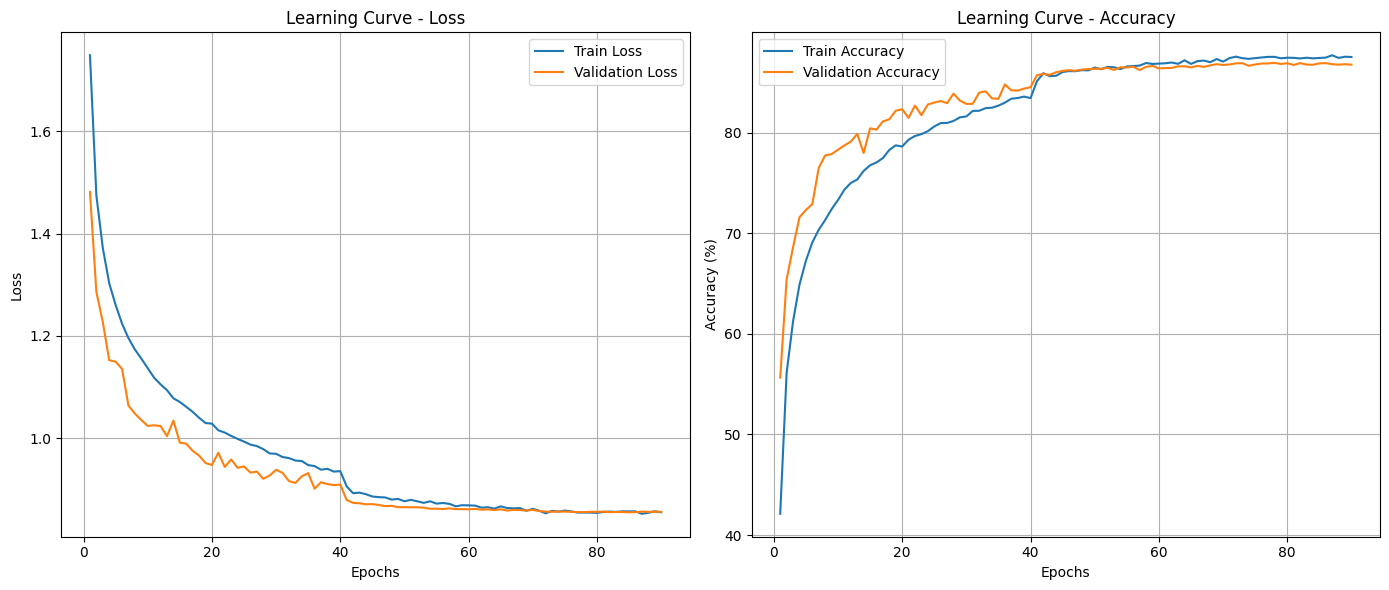
\includegraphics[width=0.9\textwidth]{learning_curves.png}
    \caption{Đường cong học tập (Loss và Accuracy).}
    \label{fig:learning_curves}
\end{figure}
Trong 40 epochs đầu, cả train loss và validation loss giảm đồng bộ, cho thấy mô hình đang học các đặc trưng hữu ích. Sau đó, dấu hiệu overfitting nhẹ xuất hiện khi train loss tiếp tục giảm nhưng validation loss dao động quanh 0.85-0.90.

Validation accuracy ổn định ở mức 86-87\% từ epoch 40-50, trong khi train accuracy tiếp tục tăng lên gần 90\%. Tuy có hiện tượng overfitting nhẹ, nhưng nhờ các kỹ thuật điều chuẩn như Dropout, Weight Decay, Label Smoothing và data augmentation, mô hình vẫn duy trì khả năng tổng quát tốt.

\section{Hiệu năng trên tập kiểm thử}
\textbf{Kết quả tổng thể} 

Mô hình đạt 86.80\% độ chính xác trên tập kiểm thử, rất gần với validation accuracy (86.89\%), chỉ chênh lệch 0.09\%. Sự nhất quán này cho thấy mô hình không bị overfitting nghiêm trọng và có khả năng tổng quát tốt.

\textbf{Hiệu suất theo từng lớp}
\begin{table}[H]
    \centering
    \caption{Độ chính xác theo từng lớp trên tập kiểm thử}
    \begin{tabular}{lc}
        \toprule
        \textbf{Lớp} & \textbf{Độ chính xác (\%)} \\
        \midrule
        Car & 94.3 \\
        Ship & 93.0 \\
        Truck & 92.0 \\
        Horse & 89.9 \\
        Frog & 89.3 \\
        Plane & 89.0 \\
        Deer & 85.7 \\
        Dog & 81.3 \\
        Bird & 80.2 \\
        Cat & 73.3 \\
        \bottomrule
    \end{tabular}
    \label{tab:class_accuracy}
\end{table}
Nhóm dẫn đầu là các phương tiện giao thông (car, ship, truck) với độ chính xác trên 92\%. Những đối tượng này có hình dạng đặc trưng rõ ràng và ít biến thể, dễ phân biệt với các lớp khác. Nhóm thách thức hơn là các động vật, đặc biệt là bộ ba cat, bird, dog. Nguyên nhân là sự đa dạng lớn về tư thế, góc nhìn, màu sắc trong cùng một lớp, và nhiều đặc điểm chung giữa các loài.

\section{Phân tích ma trận nhầm lẫn}
\begin{figure}[H]
    \centering
    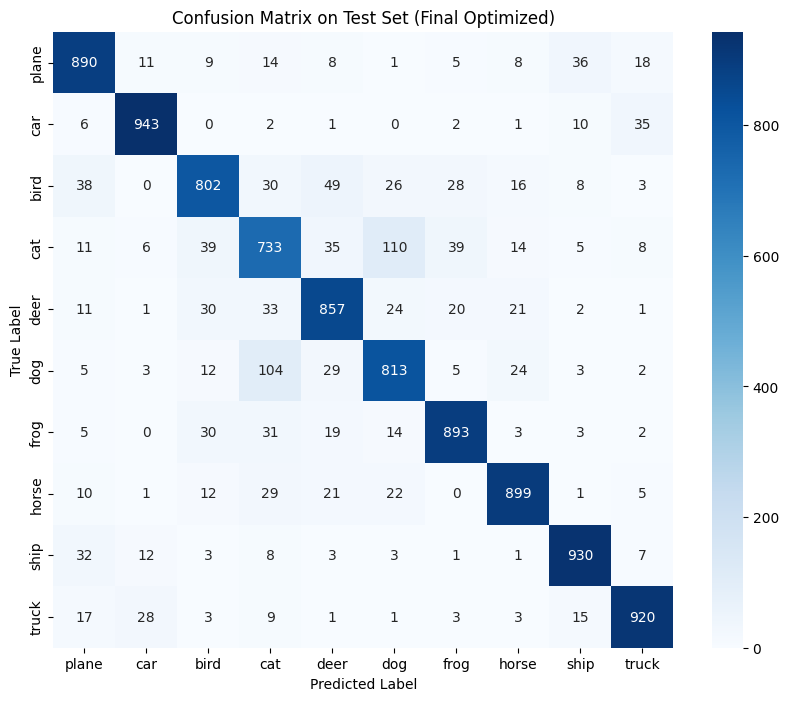
\includegraphics[width=0.7\textwidth]{confusion_matrix.png}
    \caption{Ma trận nhầm lẫn trên tập kiểm thử.}
    \label{fig:confusion_matrix}
\end{figure}
Các cặp nhầm lẫn chính:
\begin{itemize}
    \item cat $\leftrightarrow$ dog: 214 trường hợp (110 + 104) - cặp nhầm lẫn nhiều nhất
    \item bird $\rightarrow$ deer: 49 trường hợp
    \item deer $\rightarrow$ cat: 33 trường hợp
    \item bird $\rightarrow$ cat: 30 trường hợp
\end{itemize}

Cặp cat-dog nhầm lẫn nhiều nhất là điều dễ hiểu vì cả hai đều là động vật bốn chân, có lông, có tai nhọn. Trong không gian 32x32 pixel của CIFAR-10, các chi tiết phân biệt tinh tế có thể bị mất đi. Bird xuất hiện trong nhiều cặp nhầm lẫn khác nhau, cho thấy trong không gian đặc trưng mà mô hình học được, một số hình ảnh chim có đặc điểm chung với các động vật khác ở những góc chụp nhất định.

\section{Đánh giá chung}
Sau quá trình huấn luyện và đánh giá, mô hình Mạng Nơ-ron Tích Chập (CNN) đã cho thấy hiệu năng đáng kể trên bộ dữ liệu CIFAR-10, đạt độ chính xác tổng thể 86.80\% trên tập kiểm thử. Kết quả này phản ánh sự thành công trong việc tích hợp các kỹ thuật huấn luyện hiện đại như tăng cường dữ liệu đa dạng, các phương pháp điều chuẩn hiệu quả, cùng với cơ chế tự động điều chỉnh tốc độ học và dừng sớm. Mô hình đã chứng tỏ khả năng tổng quát hóa tốt, thể hiện qua sự nhất quán giữa hiệu suất trên tập kiểm định và tập kiểm thử, đồng thời cho thấy hiệu suất vượt trội khi phân loại các lớp đối tượng có đặc trưng hình ảnh rõ ràng như phương tiện giao thông ('car', 'ship', 'truck').

Tuy nhiên, sau khi phân tích kết quả nhận được chi tiết, em cũng nhận ra một số hạn chế. Hiện tượng overfitting nhẹ vẫn còn quan sát được qua đường cong học tập, cho thấy vẫn cần cải thiện thêm về khả năng tổng quát hóa. Bên cạnh đó, mô hình gặp nhiều khó khăn hơn trong việc phân biệt các lớp động vật có đặc điểm thị giác tương đồng cao (ví dụ: 'cat' và 'dog'), với độ chính xác thấp hơn đáng kể so với các lớp khác. Điều này cho thấy kiến trúc CNN 3 lớp hiện tại, dù hiệu quả, có thể chưa đủ năng lực để nắm bắt những khác biệt tinh vi giữa các lớp phức tạp này.

Như vậy, mô hình CNN hiện tại mà em đã xây dựng là một nền tảng vững chắc, thể hiện sự thành công trong việc áp dụng các nguyên lý học sâu. Những phân tích về điểm mạnh và hạn chế mà em thực hiện không chỉ khẳng định những gì mô hình CNN đã đạt được mà còn giúp em vạch ra lộ trình rõ ràng cho các bước tối ưu hóa và nâng cao hiệu suất trong tương lai. Điều này sẽ hướng em tới việc giải quyết hiệu quả hơn những thách thức còn tồn tại trong bài toán phân loại ảnh phức tạp, đặc biệt là với những đối tượng có đặc trưng tương đồng cao như các loài động vật.

\end{document}